\documentclass[letterpaper,11pt]{article}

% Soporte para los acentos.
\usepackage[utf8]{inputenc}
\usepackage[T1]{fontenc}    
% Idioma español.
\usepackage[spanish,mexico, es-tabla]{babel}
% Soporte de símbolos adicionales (matemáticas)
\usepackage{multirow}
\usepackage{amsmath}		
\usepackage{amssymb}		
\usepackage{amsthm}
\usepackage{amsfonts}
\usepackage{latexsym}
\usepackage{enumerate}
\usepackage{ragged2e}
\usepackage{graphicx}
\usepackage{hyperref}
\usepackage{caption}
\usepackage{subcaption}
% Modificamos los márgenes del documento.
\usepackage[lmargin=2cm,rmargin=2cm,top=2cm,bottom=2cm]{geometry}

\title{Facultad de Ciencias, UNAM \\ 
       Reconocimiento de patrones y aprendizaje automatizado \\ 
       Tarea 2}
\author{Rubí Rojas Tania Michelle}
\date{\today}

\begin{document}
\maketitle

\begin{enumerate}
    % Ejercicio 1.
    \item Cada una de las líneas en el documento \texttt{tarea2\_docs.txt} lo 
    vamos a considerar como un documento. Realiza la limpieza y preprocesamiento 
    necesarios.

    \textsc{Solución:} Leemos el archivo \textbf{tarea\_docs.txt} línea por 
    línea (ya que cada una de éstas será considerada como un documento) y lo 
    guardamos en un arreglo. Posteriormente, convertimos este arreglo en un 
    \texttt{DataFrame} cuya única columna se llamará \texttt{'text'} y cada una 
    de sus filas contendrá los distintos textos guardados.
    \begin{center}
        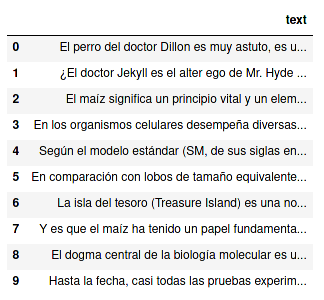
\includegraphics[width=0.4\textwidth]{imagenes/text1.png}
    \end{center}

    Luego, convertimos cada uno de los documentos en vectores usando TFIDF.
    \begin{center}
        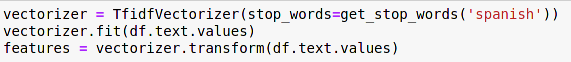
\includegraphics[width=0.65\textwidth]{imagenes/text2.png}
    \end{center}

    Por otro lado, usaremos el algoritmo \textbf{K-means} para agrupar nuestros 
    datos. De esta forma, para encontrar el valor adecuado de $K$ realizamos una 
    gráfica e intenamos hallar el \textit{Elbow Curve}, para lo cual ejecutamos 
    varios \textit{k-means}, incrementamos a $k$ en cada iteración y registramos 
    el valor del SSE.
    \begin{center}
        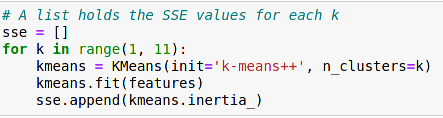
\includegraphics[width=0.45\textwidth]{imagenes/text4.png}
    \end{center}
    \newpage
    \begin{center}
        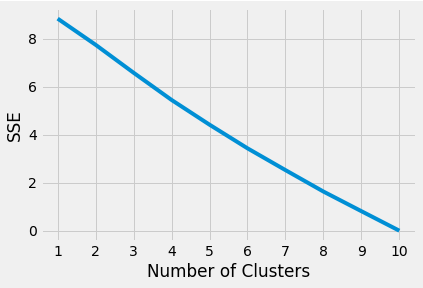
\includegraphics[width=0.35\textwidth]{imagenes/text3.png}
    \end{center}

    donde podemos notar que en $k=5$ se dobla ligeramente la curva. Así, 
    ejecutamos \textbf{K-means} con este valor, realizamos nuestras predicciones 
    y modificamos el \texttt{DataFrame} de tal forma que agregamos la nueva 
    clasificación encontrada.
    \begin{center}
        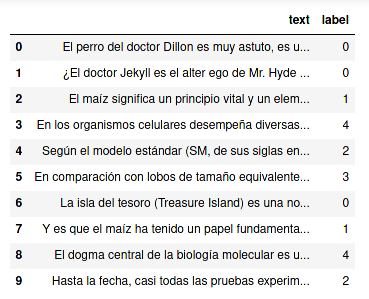
\includegraphics[width=0.45\textwidth]{imagenes/text5.png}
    \end{center}

    Como podemos observar, los textos se clasificaron en $5$ grupos diferentes. 
    Separamos cada texto en un \texttt{DataFrame} distinto para poder visualizar 
    los resultados.
    \begin{figure}[ht]
        \centering
        {{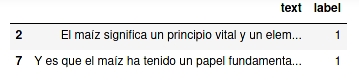
\includegraphics[width=0.4\textwidth]{imagenes/text7.png}}}%
        \qquad
        {{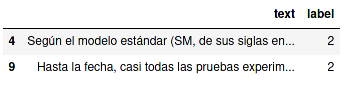
\includegraphics[width=0.4\textwidth]{imagenes/text8.png}}}%
    \end{figure}
    \begin{figure}[ht]
        \centering
        {{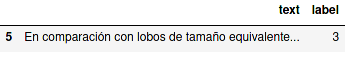
\includegraphics[width=0.4\textwidth]{imagenes/text9.png}}}%
        \qquad
        {{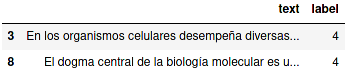
\includegraphics[width=0.4\textwidth]{imagenes/text10.png}}}%
    \end{figure}
    \begin{figure}[ht]
        \centering
        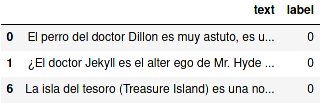
\includegraphics[width=0.4\textwidth]{imagenes/text6.png}
    \end{figure}

    Podemos observar que obtuvimos una muy buena agrupación, pues a mi 
    consideración, sólo agrupó erróneamente un texto (y se encuentra en el 
    grupo $3$).
    
    \newpage
    Contesta las siguientes preguntas:
    \begin{itemize}
        % Ejercicio 1.a
        \item ¿En qué tópicos se pueden dividir?

        \textsc{Solución:} Se puede dividir en $5$ diferentes tópicos:
        \begin{itemize}
            \item Aquellos con la etiqueta $1$, que corresponden a temas 
            relacionados con el maíz en los pueblos indígenas y la cultura 
            mexicana.

            \item Aquellos con la etiqueta $2$, que corresponden a temas 
            relacionados con la física.

            \item Aquel con la etiqueta $3$, que corresponde a la descripción 
            de lobos (el cual debería de estar relacionado con el texto que 
            habla del perro del Doctor Dillon, pues hablan de cosas similares).

            \item Aquellos con la etiqueta $4$, que corresponden a temas de 
            biología molecular.

            \item Aquellos con la etiqueta $0$, que corresponden a descripciones
            de libros (con un integrante erróneo).
        \end{itemize}

        % Ejercicio 1.b
        \item ¿Qué documentos habla de México y su cultura?

        \textsc{Solución:} Los documentos etiquetados con el número $1$.
    \end{itemize}

    % Ejercicio 2.
    \item Descarga el dataset de datos de sonar de la siguiente liga:
    \url{https://archive.ics.uci.edu/ml/machine-learning-databases/undocumented/
    connectionist-bench/sonar/sonar.all-data}

    Mismo que deberás explorar y entender lo que hacen sus atributos. 
    
    Lleva a cabo una clasificación utilizándo la regresión logística de los 
    datos. Luego, efectúa una reducción de dimensión y haz tu clasificación 
    otra vez. La comparación entre las clasificaciones la harás con las 
    métricas que tú elijas. 

    ¿Qué observas y por qué sucede esto?

    \textsc{Solución:} \textbf{sonar.all-data} es un conjunto de datos que 
    describe el sonido (o más bien, el chirrido) del sonar al rebotar sobre 
    diferentes superficies. Las $59$ variables de entrada son la fuerza de los 
    retornos en ángulos diferentes y se encuentran en un rango de $0$ a $1$. La 
    variable $60$ de salida es un string \textbf{M} para Mina y \textbf{R} para 
    Roca.

    El problema es de clasificación binaria, la cual requiere de un modelo para 
    diferenciar rocas de cilindros metálicos.

    Descargamos el conjunto de datos y lo visualizamos.
    \begin{center}
        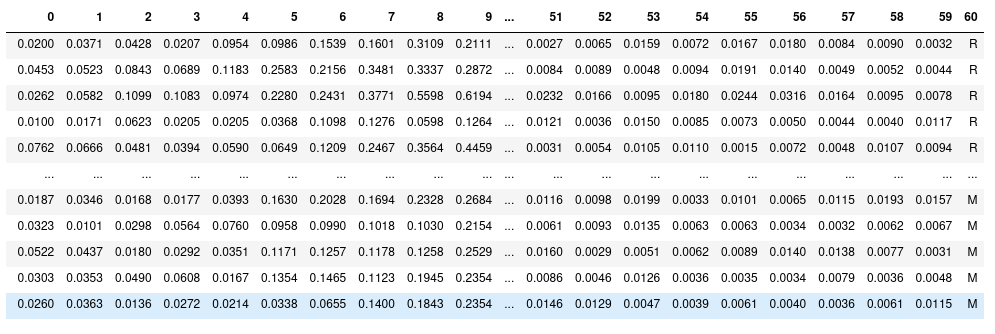
\includegraphics[width=0.9\textwidth]{imagenes/sonar-dataset.png}
    \end{center}

    \newpage
    Veamos si la proporción de los datos en cada clase es equilibrada.
    \begin{center}
        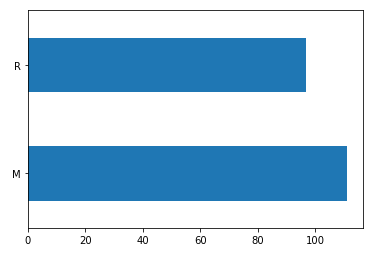
\includegraphics[width=0.3\textwidth]{imagenes/sonar-equilibrio.png}
    \end{center}

    donde existen $111$ datos para la clase Mina y $97$ datos para la clase 
    Roca. Como no hay mucha diferencia entre ambas clases, entonces no es 
    necesario rebalancear de alguna manera el conjunto de datos. 

    Aunque los metadatos dicen que todos los predictores van de $0$ a $1$, 
    todavía encontramos que hay varios de ellos que tienen valores relativamente
    menores en comparación con la mayoría. También encontramos que no hay
    ningún valor alto más grande que $1$.
    \begin{center}
        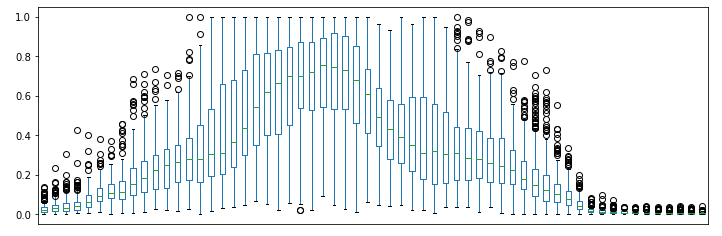
\includegraphics[width=0.5\textwidth]{imagenes/sonar-boxes.png}
    \end{center}

    La matriz de correlación nos indica que hay alguna estructura en el órden 
    de los atributos: el color rojo alrededor de la diagonal sugiere que los 
    atributos que están uno al lado del otro están más correlacionados entre 
    sí (es decir, cada variable tiene una gran correlación positiva con sus 
    vecinos), las manchas azules sugieren alguna correlación negativa moderada 
    entre los atributos que están más alejados unos de otros. Esto tiene 
    sentido si el órden de los atributos se refiere al ángulo de los sensores 
    para el chirrido del sonar.
    \begin{center}
        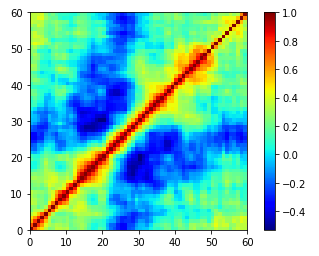
\includegraphics[width=0.25\textwidth]{imagenes/sonar-correlacion.png}
    \end{center}

    Ahora bien, para el procesamiento de datos separamos al conjunto de datos 
    en dos:
    \begin{itemize}
        \item $X$: el cual está conformado por las primeras $59$ columnas del 
        dataset original.
        \item $y$: el cual está conformado por la columna $60$ del dataset 
        original.
    \end{itemize}

    La gráfica de cajas nos sugiere que debemos estandarizar los datos de 
    entrada, por lo que usamos la clase \textbf{StandardScaler} para lograr 
    esto (recordándo que ésta elimina la media y escala los datos de forma que 
    su varianza sea igual a $1$). 

    La variable de salida (la columna $60$) es un string \textbf{M} o \textbf{R}.
    Debemos convertirlos en valores enteros entre $0$ y $1$, y para lograr esto 
    usamos la clase \textbf{LabelEncoder} (la cual modelará la codificación 
    requerida usando todo el conjunto de datos a traves de la función 
    \texttt{fit()} y luego aplicará la codificación para crear una nueva variable 
    de salida usando la función \texttt{transform()}).

    Para crear el modelo de regresión lineal, dividimos nuestro conjunto de datos 
    ya modificado en entrenamiento ($80\%$) y prueba ($20\%$). Luego, simplemente 
    creamos una instancia de \\ 
    \texttt{LogisticRegression}  y lo entrenamos.

    Los resultados obtenidos fueron los siguientes:
    \begin{center}
        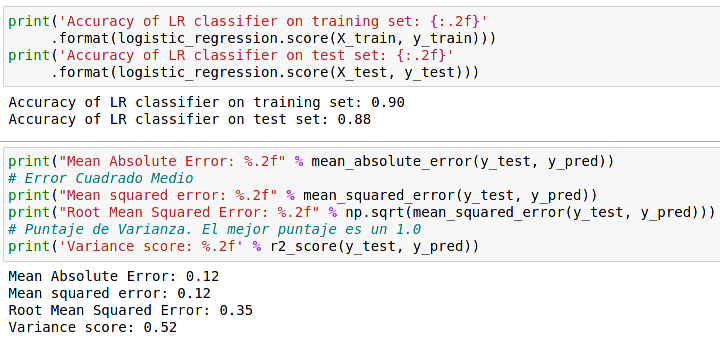
\includegraphics[width=0.8\textwidth]{imagenes/sonar-lg1.png}
        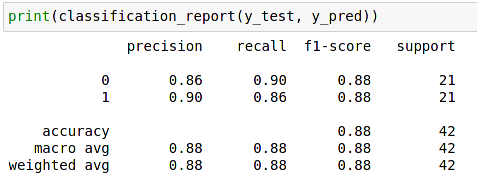
\includegraphics[width=0.5\textwidth]{imagenes/sonar-lg2.png}
    \end{center}

    donde en particular podemos notar que 
    \begin{itemize}
        \item Obtenemos un $90\%$ de precisión en el conjunto de entrenamiento 
        y un $88\%$ de precisión en el conjunto de prueba.

        \item Obtenemos MSE de $0.12$ (con un puntaje de varianza de $0.52$).

        \item Obtenemos $86\%$ de precisión para los datos correspondientes a 
        metales y $90\%$ de precisión para los datos correspondientes a las 
        rocas.
    \end{itemize}
    
    Por otro lado, usaremos PCA para obtener la lista de atributos que tienen 
    mayor varianza (mayor poder explicativo). Éstos serán los componentes 
    principales. Realizamos un par de gráficas para poder determinar el 
    número de estos componentes.
    \begin{figure}[ht]
        \centering
        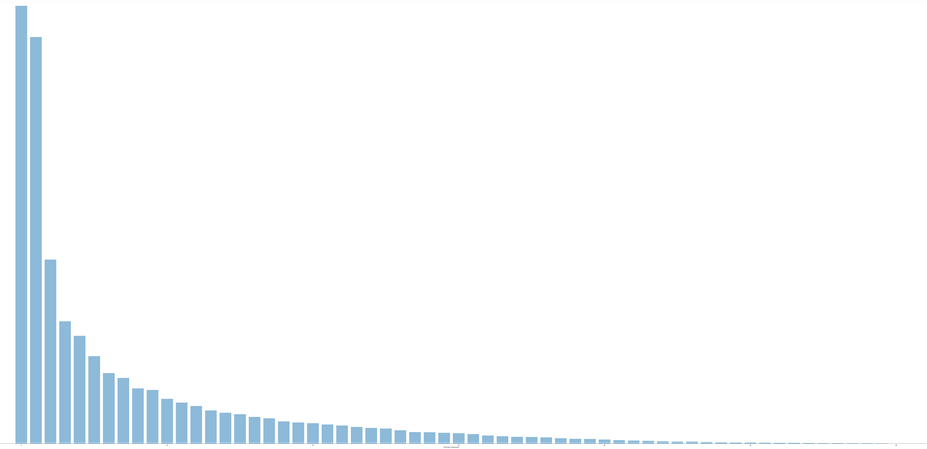
\includegraphics[width=0.7\textwidth]{imagenes/sonar-pca1.png}
        \caption{Variance Ratio vs Principal componentes }
    \end{figure}
    \begin{figure}[ht]
        \centering
        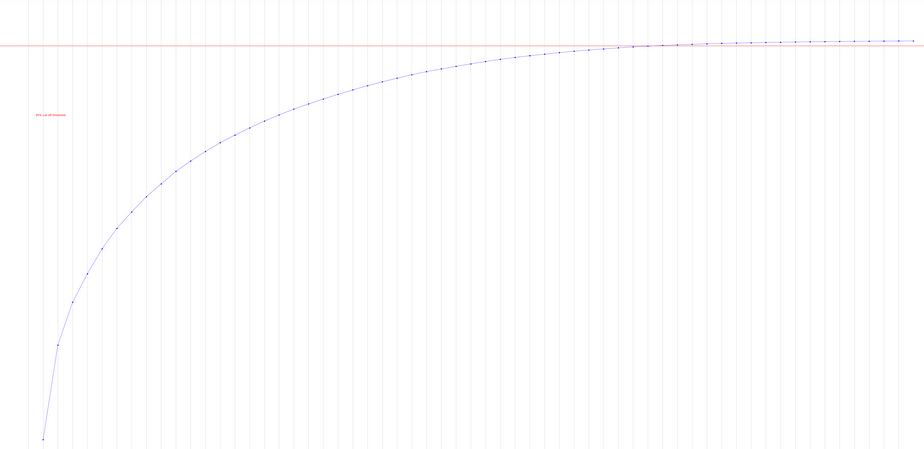
\includegraphics[width=0.8\textwidth]{imagenes/sonar-pca2.png}
        \caption{Cumulative variance vs Number of Components}
    \end{figure}

    Donde obtenemos que con $43$ componentes tenemos un $99\%$ de la 
    varianza explicada (queremos una v.e. entre $95\%$ y $99\%$, pero me ha 
    gustado más al resultado con este valor). Así, creamos una instancia 
    de PCA con un número de $43$ componentes principales y la entrenamos, 
    para después pasarle este nuevo conjunto $X\_pca$ al modelo de 
    \texttt{LogisticRegression} y entrenarlo.

    Los resultados obtenidos fueron los siguientes:
    \begin{center}
        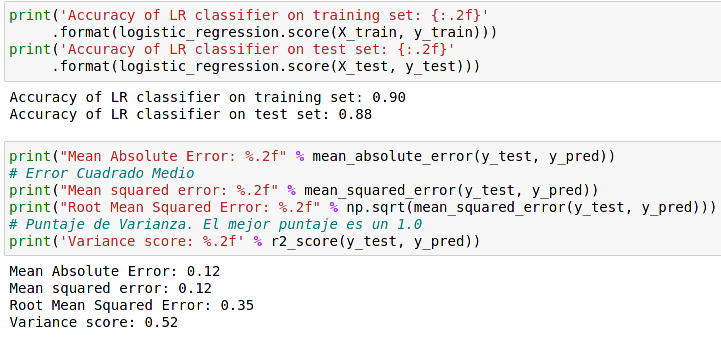
\includegraphics[width=0.8\textwidth]{imagenes/sonar-pca3.png}
        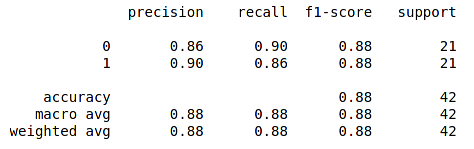
\includegraphics[width=0.5\textwidth]{imagenes/sonar-pca4.png}
    \end{center}

    donde en particular podemos notar que 
    \begin{itemize}
        \item Obtenemos un $90\%$ de precisión en el conjunto de entrenamiento 
        y un $88\%$ de precisión en el conjunto de prueba.

        \item Obtenemos MSE de $0.12$ (con un puntaje de varianza de $0.52$).

        \item Obtenemos $86\%$ de precisión para los datos correspondientes a 
        metales y $90\%$ de precisión para los datos correspondientes a las 
        rocas.
    \end{itemize}

    Así, podemos concluir que obtenemos la misma precisión que en el modelo 
    anterior usando $43$ componentes principales ($16$ columnas menos). Esto 
    puede ser causado por el nivel de correlación que notamos al analizar los 
    datos.

    % Ejercicio 3.
    \item Diseña un experimento para determinar para qué umbral es posible tener 
    un conjunto de datos no balanceado.

    \textsc{Solución:} Utilizamos la clase \texttt{make\_classification}, la 
    cual genera conjuntos de datos a partir de ciertos parámetros que nosotros 
    podemos modificar. Al crear $9$ distintos datsets, obtenemos las siguientes 
    gráficas:
    \begin{figure}[ht]
        \centering
        \subfloat[\texttt{100 datos con \{900, 100\}}]
        {{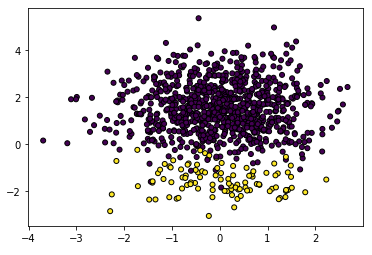
\includegraphics[width=0.35\textwidth]{imagenes/experimento1.png}}}
        \qquad
        \subfloat[\texttt{1000 datos con \{75, 25\}}]
        {{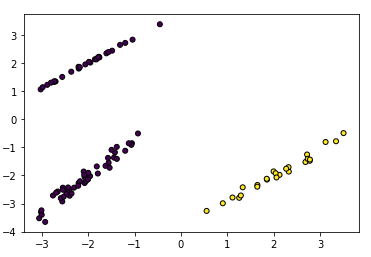
\includegraphics[width=0.35\textwidth]{imagenes/experimento2.png}}}
    \end{figure}
    \begin{figure}[ht]
        \centering
        \subfloat[\texttt{10000 datos con \{6000, 4000\}}]
        {{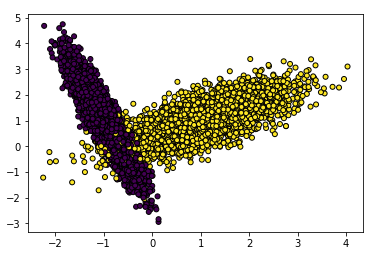
\includegraphics[width=0.35\textwidth]{imagenes/experimento3.png}}}
        \qquad
        \subfloat[\texttt{1000 datos con \{997, 3\}}]
        {{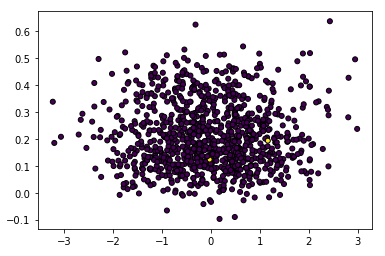
\includegraphics[width=0.35\textwidth]{imagenes/experimento4.png}}}
    \end{figure}
    \begin{figure}[ht]
        \centering
        \subfloat[\texttt{200 datos con \{11, 189\}}]
        {{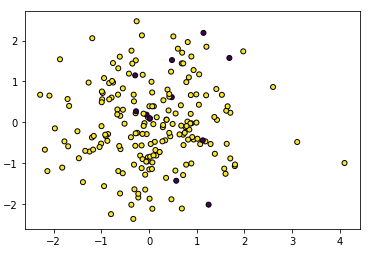
\includegraphics[width=0.35\textwidth]{imagenes/experimento5.png}}}
        \qquad
        \subfloat[\texttt{200 datos con \{57, 130, 13\}}]
        {{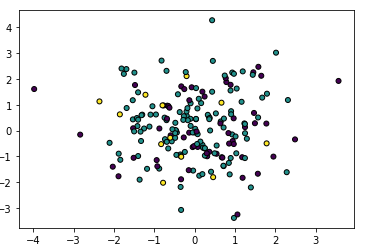
\includegraphics[width=0.35\textwidth]{imagenes/experimento6.png}}}
    \end{figure}
    \begin{figure}[ht]
        \centering
        \subfloat[\texttt{1000 datos con \{227, 47, 726\}}]
        {{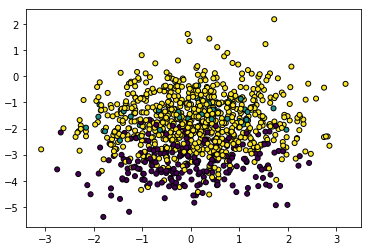
\includegraphics[width=0.35\textwidth]{imagenes/experimento7.png}}}
        \qquad
        \subfloat[\texttt{3575 datos con \{1630, 1945\}}]
        {{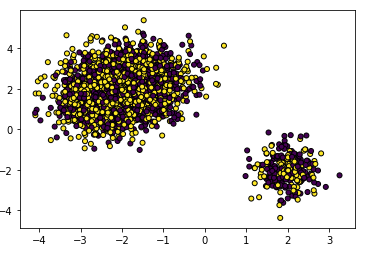
\includegraphics[width=0.35\textwidth]{imagenes/experimento8.png}}}
    \end{figure}

    \newpage
    Ahora bien, al estar jugando con varios de los parámetros notamos que 
    aquellos que verdaderamente influyen para que un conjunto de datos sea 
    desbalanceado son \textbf{flip\_y} y \textbf{weights} mientras que el resto 
    de los parámetros sólo parecen influir en las características de los datos 
    (más no en la distribución de valores en cada clase).

    El parámetro \textbf{weight} sirve para poder asignar la proporción de 
    valores que tendrá cada una de las clases. De esta forma, si queremos un 
    conjunto de datos desbalanceado, debemos ajustar estos valores para que 
    así sea.  Por ejemplo, si tenemos $100$ datos y queremos una proporción 
    $60-40$ (y tenemos dos clases) entonces debemos escribir 
    \texttt{weight[0.6,0.4]}.

    La suma de las proporciones no debe ser necesariamente $1$, y en algunos 
    casos, cuando este valor es mayor a $1$, se regresan más valores de lo 
    que deberían (y en un experimento pudimos ver que todas las clases toman 
    casi los mismos valores cuando esto pasa).

    En particular, encontramos que si \textbf{flip\_y} es mayor a $0$ entonces 
    lo que hace es ir aumentando los valores de las clases (como si se estuviera 
    balanceando) poco a poco. Con un valor \textbf{flip\_y < 0.5} realmente el 
    conjunto sigue desbalanceado, pero conforme el valor se acerca a $1$ entonces
    los valores de las clases se van \textit{balanceando}. Esto último lo podemos 
    ver con el siguiente conjunto
    \begin{verbatim}
        X8, y8 = make_classification(flip_y=1, n_informative=2, n_repeated=0,
                                     n_clusters_per_class=1, n_samples=4000, 
                                     shuffle=True, n_features=2, n_redundant=0, 
                                     random_state=7, class_sep=2, n_classes=2, 
                                     weights=[0.1, 0.9])
    \end{verbatim}

    donde podemos observar que a pesar de que las proporciones de los datos son 
    \texttt{1:9}, gracias a que el valor de \textbf{flip\_y} es igual a $1$, las 
    proporciones de las clases son totalmente diferentes (pues obtenemos que 
    los valores son \texttt{\{2065, 1935\}})
    \begin{figure}[ht]
        \centering
        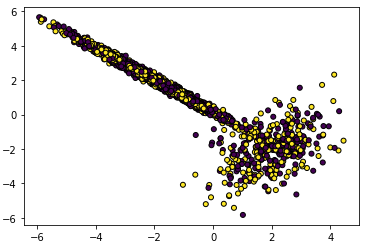
\includegraphics[width=0.4\textwidth]{imagenes/experimento9.png}
    \end{figure}

    \newpage
    Creo además que el número de clusters también puede influir, pero realmente 
    desvía los valores de las clases muy pero muy poquito, entonces no afecta 
    mucho en el umbral que buscamos.

    % Ejercicio 4.
    %\item Reproduce la gráfica de la información mutua del seno contra él mismo 
    %considerándo un corrimiento de $50$ posiciones.

    % Ejercicio 5.
    \item El dataset de \texttt{seatbelt.csv} representa una serie de datos 
    temporales de diversos atributos que hacen referencia a la mortalidad 
    asociada a los accidentes de tránsito en Gran Bretaña en el periodo de 
    $1969$ y $1984$. La legislación para utilizar el cinturón de seguridad de 
    manera obligatoria fue introducida el $31$ de enero de $1983$. Ajusta un 
    modelo lineal generalizado para determinar la probabilidad de morir en 
    un accidente de tránsito. Se espera que lleves a cabo la normalización o 
    estandarización del dataset, la transformación de las variables que 
    consideres pertinente y que propongas qué variables tienen más o menos 
    importancia en la probabilidad de morir en un accidente de tránsito.
    Responde las siguientes preguntas:
    \begin{itemize}
        % Ejercicio 5.a
        \item ¿Volver obligatorio el cinturón de seguridad disminuyó la 
        probabilidad de morir en algún accidente de tránsito?

        % Ejercicio 5.b
        \item ¿Qué otra conclusión puedes generar a partir del modelo que 
        ajustaste?
    \end{itemize} 

    \textsc{Solución:} Notemos que nuestro conjunto de datos se ve de la 
    siguiente forma:
    \begin{center}
        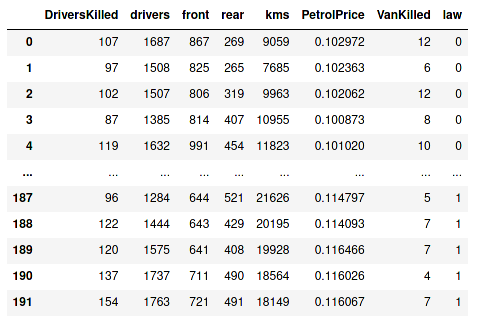
\includegraphics[width=0.5\textwidth]{imagenes/seat1.png}
    \end{center}

    el cual contiene $192$ entradas y $8$ atributos. Como la tarea principal 
    del conjunto de datos se centrará en el antes y el después de la 
    introducción de la legislación sobre el cinturón de seguridad, es 
    conveniente dividir el conjunto de datos en dos: 
    \begin{itemize}
        \item Uno antes de la legislación (\texttt{law=0}) y, 
        \item Otro después de la legislación (\texttt{law=1})
    \end{itemize}

    Contando el número de entradas en cada uno de estos conjuntos obtenemos que 
    hay $169$ entradas para \texttt{law=0}, mientras que \texttt{law=1} tiene 
    únicamente $23$ entradas.
    \begin{center}
        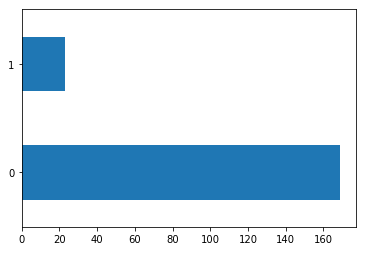
\includegraphics[width=0.35\textwidth]{imagenes/seat2.png}
    \end{center}

    Luego, vemos la proporción de conductores fallecidos antes y después de que 
    usar cinturón de seguridad fuera obligatorio.
    \begin{itemize}
        \item Pasajeros al frente y detrás:
        \begin{itemize}
            \item Sin ley, la probabilidad es de $0.7415$.
            \item Con ley, la probabilidad es de $0.6169$.
        \end{itemize}

        \item Pasajeros al frente:
        \begin{itemize}
            \item Sin ley, la probabilidad es de $0.5084$.
            \item Con ley, la probabilidad es de $0.4319$.
        \end{itemize}

        \item Pasajeros detrás:
        \begin{itemize}
            \item Sin ley, la probabilidad es de $0.2330$.
            \item Con ley, la probabilidad es de $0.3084$.
        \end{itemize}
    \end{itemize}

    Por lo tanto, podemos concluir que efectivamente disminuyó la probabilidad 
    de morir en un accidente de auto. Podemos notar además que la probabilidad
    de morir siendo pasajero detrás aumentó con la legislación.

    Por otro lado, para calcular la correlación y la regresión lineal entre dos 
    factores se utilizó el conjunto de datos \textbf{sinley} (pues tiene la 
    mayor cantidad de entradas), esto para que los datos no estuvieran sesgados 
    por los diferentes factores.

    De esta forma, procedemos a calcular la correlación entre los atributos. 
    \begin{itemize}
        \item Kilometraje vs Precio de la gasolina
        
        Obtenemos una correlación de $0.2454$.
        \begin{center}
            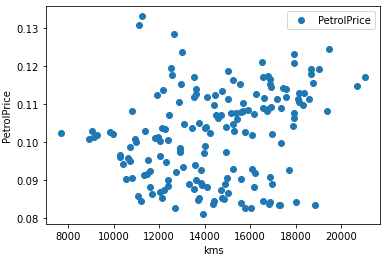
\includegraphics[width=0.4\textwidth]{imagenes/seat3.png}
        \end{center}

        Donde, a pesar de esperar que la correlación fuera negativa (pues a 
        mayor precio de la gasolina, menos distancia se recorrería); se obtuvo 
        un valor positivo.

        \newpage
        \item Pasajeros al frente vs número de fallecidos.

        Obtenemos una correlación de $0.6808$.
        \begin{center}
            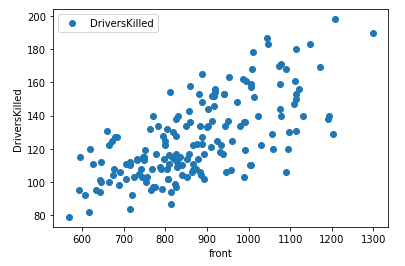
\includegraphics[width=0.4\textwidth]{imagenes/seat4.png}
        \end{center}

        \item Pasajeros en los asientos traseros vs número de fallecidos.

        Obtenemos una correlación de $0.6981$.
        \begin{center}
            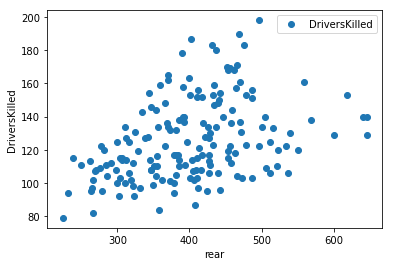
\includegraphics[width=0.4\textwidth]{imagenes/seat5.png}
        \end{center}

        \item Kilometraje vs número de fallecidos.

        Obtenemos una correlación de $-0.1914$.
        \begin{center}
            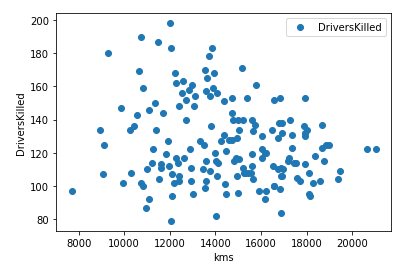
\includegraphics[width=0.4\textwidth]{imagenes/seat6.png}
        \end{center}

        \item Precio de la gasolina vs número de fallecidos.

        Obtenemos una correlación de $-0.3120$.
        \begin{center}
            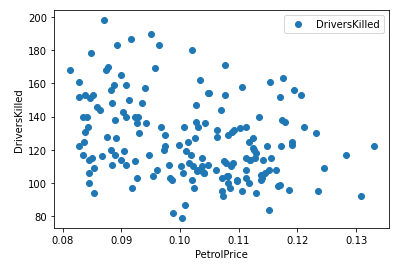
\includegraphics[width=0.35\textwidth]{imagenes/seat7.png}
        \end{center}

        \item Número de furgonetas vs número de fallecidos.

        Obtenemos una correlación de $0.3382$.
        \begin{center}
            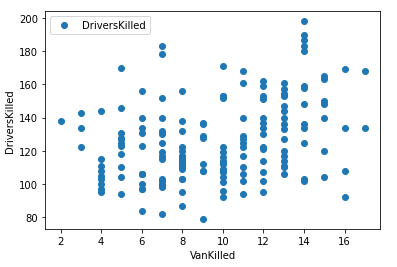
\includegraphics[width=0.4\textwidth]{imagenes/seat8.png}
        \end{center}
    \end{itemize}

    Notemos que las variables independientes parecen ser Kms, PetrolPrice, 
    Front y Rear, mientras que la variable dependiente será DriversKilled.

    Después, definimos dos nuevos conjuntos:
    \begin{itemize}
        \item $X$: correspondiente a las variables independientes.
        \item $y$: correspondiente a la variable dependiente.
    \end{itemize}

    Y separamos nuestro conjunto en prueba y entrenamiento en un $20-80$, 
    respectivamente. Creamos una instancia del algoritmo 
    \texttt{LinearRegression}, y lo entrenamos.

    Los coeficientes obtenidos son:
    \begin{center}
        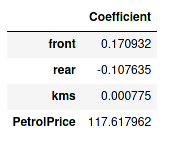
\includegraphics[width=0.25\textwidth]{imagenes/seat9.png}
    \end{center}

    Esto significa que, 
    \begin{itemize}
        \item Cuando \texttt{DriverKilled} incrementa una unidad, entonces 
        \texttt{front} incrementa $0.170932$ unidades.

        \item Cuando \texttt{DriverKilled} incrementa una unidad, entonces 
        \texttt{rear} disminuye $-0.107635$ unidades.

        \item Cuando \texttt{DriverKilled} incrementa una unidad, entonces 
        \texttt{kms} incrementa $0.000775$ unidades.

        \item Cuando \texttt{DriverKilled} incrementa una unidad, entonces 
        \texttt{PetrolPrice} incrementa $117.617962$ unidades.
    \end{itemize}

    \newpage
    Realizando nuestras predicciones, obtenemos los siguientes resultados:
    \begin{center}
        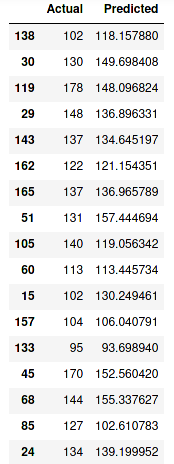
\includegraphics[width=0.25\textwidth]{imagenes/seat10.png}
    \end{center}

    y visualizamos la precisión de nuestro modelo:
    \begin{center}
        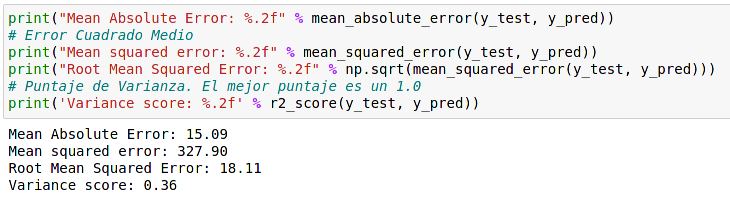
\includegraphics[width=0.8\textwidth]{imagenes/seat11.png}
    \end{center}

    A partir de esto, podemos concluir que el modelo realiza predicciones 
    considerablemente buenas. 
\end{enumerate}

\end{document}
